\documentclass[12pt,a4paper]{article}
\usepackage[utf8]{inputenc}
\usepackage{amsmath}
\usepackage{amsfonts}
\usepackage{amssymb}
\usepackage{amsthm}
\usepackage[left=2cm,right=2cm,top=2cm,bottom=2cm]{geometry}
\usepackage{enumitem}
\usepackage{tikz}
\usepackage{tikz-cd}
\usepackage{url}

\title{Mathematical software - homework 2}
\author{Sebastiano Tronto}

\newtheorem{thm}{Theorem}
\newtheorem{prop}[thm]{Proposition}

\theoremstyle{definition}
\newtheorem{ex}{Exercise}

\theoremstyle{definition}
\newtheorem*{remark}{Remark}

\newcommand{\bs}{\textbackslash}

\begin{document}

\noindent\hrulefill

\begin{center}
\Huge{\textbf{Mathematical Software - Homework 2}}
\end{center}

\noindent\hrulefill
\begin{center}
\begin{tabular}{lcr}
\texttt{sebastiano.tronto@uni.lu} & \qquad \qquad \qquad \qquad &
\textbf{Deadline: Sunday, April 18th}
\end{tabular}
\end{center}

\vspace{1cm}

\begin{center}
  \emph{\large
    For each of the following exercises submit a .tex and a .pdf file.
  }
\end{center}

\vspace{1cm}

\begin{ex}
  Create a Latex document containing the following pictures:
  \begin{enumerate}[label=(\alph*)]
    \item The regular polygon with $N$-sides centered at the origin of the
          plane (see below).
          The number $N$ of sides must be easy to change at will: you should
          use the \texttt{\textbackslash pgfmathsetmacro} command to set a
          value for $N$ at the beginning, so that changing only that number
          makes the whole picture change accordingly.
      \begin{center}
        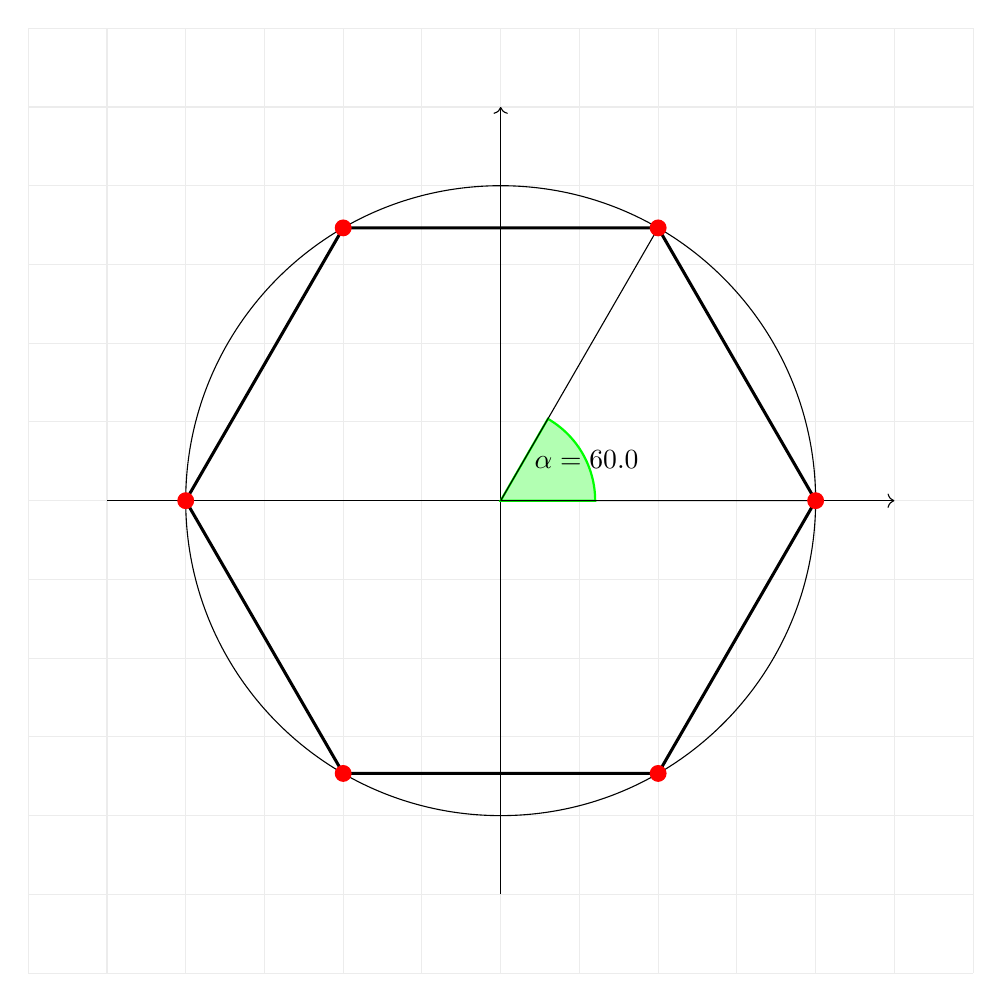
\begin{tikzpicture}[scale=1]
        	\pgfmathsetmacro{\N}{6}	
        	\pgfmathsetmacro{\an}{360/\N}
        	\pgfmathsetmacro{\r}{4}
	
        	\draw[lightgray!30,thin] (-6,-6) grid (6,6);
        	\draw[->] (-5,0) -- (5,0);
        	\draw[->] (0,-5) -- (0,5);

        	\filldraw[draw=green,fill=green!30,thick] (0.3*\r,0)
        	  arc[radius=0.3*\r,start angle=0, end angle=\an]
        	  -- node[right] {$\alpha=\an$}(0,0) --  cycle;
        	\draw[thin] (\an:\r) -- (0,0) circle[radius=\r] -- (\r,0);
        	\draw[line width=1.1pt]
        	  (\r,0)  \foreach \x in {1,2,...,\N} { -- (\x*\an:\r) };
        	\foreach \x in {1,...,\N} {
        		\filldraw[red] (\x*\an:\r) circle[radius=0.1];
        	};
        \end{tikzpicture}
      \end{center}
    \item The following commutative diagram:
      \begin{tikzcd}
        0 \ar[r] & A' \ar[r,hook] \ar[d] & A \ar[r,two heads] \ar[d,"\sim"] &
          A'' \ar[r] \ar[d] \ar[l,dashed,"s"',bend right] & 0 \\
        0 \ar[r] & A' \ar[r,hook,"i_{A'}"'] & A'\oplus A''
          \ar[r,two heads,"\pi_{A''}"'] & A'' \ar[r] & 0 
      \end{tikzcd}
  \end{enumerate}
\end{ex}

\vspace{0.8cm}

\begin{ex}
  Suppose you have to give a short presentation (10 minutes) on a topic of
  your choice related to your study programme (you will not be asked to
  actually perform this presentation). You can choose to talk about a theorem
  you find important, a result you have seen in class or something else (see
  below for a list of possible topics). For example, if you talk about an
  important theorem you can give the theorem statement, explain why this
  theorem is important and/or possible applications of this result, and
  optionally an idea of the proof; but you can also deviate from this and talk
  for example about the historical background that lead to the development of
  this theorem.

  Your task is to prepare slides for such a presentation using Beamer (Latex).
  Since the time for the (imaginary) presentation is very short, you should
  write 5-8 slides (you can have more if some contain very few or no
  words).

  If you feel like certain slides do not make sense without your explanation
  (for example if you have one slide with just one picture and you plan to
  talk with the picture in background), you can write some comments in the
  .tex file.

  If you can't think of a topic that you like, you can pick one of the
  following:
  \begin{itemize}
    \item The fundamental theorem of arithmetic (about prime numbers)
    \item The central limit theorem (probability theory)
    \item Differential equations (what they are, applications,
          methods to solve them...)
  \end{itemize}
\end{ex}

\newpage
\section*{Grading}

This homework assignment is worth 25\% of your final grade.

\vspace{0.3cm}
\noindent\textbf{Exercise 1 (10 points).}
Part (a) is worth 5 points, divided as follows:
\begin{itemize}
  \item 3 points for obtaining a regular polygon whose number of sides
        can be changed by setting a variable with \texttt{\bs pgfmathsetmacro}
        (or in a similarly easy way).
  \item 1.5 points for other features of the picture (verteces, angle) that
        also change accordingly to the same variable.
  \item 0.5 points for the style of the other elements of the picture. This is
        a matter of personal preference and it does not need to be exactly the
        same as the picture, but some key features should remain (e.g.
        the grid lines should be less visible than the rest of the picture,
        the circle line style should be different from the polygon).
\end{itemize}
Part (b) is worth 5 points, divided as follows:
\begin{itemize}
  \item 3 points if the nodes and arrows of the diagram are correct from a
        mathematical point of view (that is, the arrows point to the correct
        object).
  \item 1 point if the labels of the arrows are placed as shown in the picture
        above.
  \item 1 point for the correct style of the arrows (dashed, curved).
\end{itemize}

\vspace{0.2cm}
\noindent\textbf{Exercise 2 (10 points).}
\begin{itemize}
  \item Producing a presentation that contains at least 4 slides is worth
        5 points (but within reason: for example, the slides must not be empty).
  \item Up to 3 more points are given if the presentation is of a suitable
        length (watch out: both a presentation too short and one too long can
        loose points!).
        Comments in the .tex file can help me understand how long you plan to
        spend on each slide. If you are not sure how long your presentation is
        going to take, try it and write down how long each slide took.
  \item Up to 2 more points will be given if the slides ``look nice'' from
        the audience's perspective (e.g. not too many words on the same slides,
        are there nice pictures, etc).
\end{itemize}


\end{document}